\section{Análisis y diseño del sistema}
\label{analisis}
\subsection{Análisis de requisitos}
\label{requisitos}

\begin{table}[H]
\centering
\begin{tabular}{|c|p{12cm}|}
\hline
\multicolumn{2}{|c|}{GUIÑOTE} \\ \hline
RF-1 &  El sistema permite a los usuarios jugar al guiñote en modo uno contra uno y dos contra dos. \\ \hline
RF-2 & El sistema almacena un historial de partidas jugadas por el usuario y permite visualizar estadísticas de las partidas jugadas. \\ \hline
RF-3 & El jugador, en mitad de una partida, puede desconectarse y   volver a conectarse desde cualquier dispositivo siempre que no sea su turno o, en caso de serlo, no agote su tiempo de turno. \\ \hline
RF-4 & El sistema requiere que los usuarios se registren con su correo electrónico o Facebook para poder acceder a los servicios que ofrece. \\ \hline
RF-5 & El jugador puede seleccionar si desea jugar una partida pública o privada. \\ \hline
RF-6 & Los usuarios pueden elegir una partida pública en curso y unirse a ella como espectadores. \\ \hline
RF-7 & El sistema cuenta con una divisa virtual que se consigue al iniciar sesión por primera vez, ganando torneos, partidas, ascensos a otra liga, etc. \\ \hline
RF-8 & El sistema consta de un panel de administración al cual se pueden conectar solamente los usuarios definidos como administradores con anterioridad. \\ \hline
RF-9 & El sistema permite al usuario administrar sus datos personales almacenados en el sistema: nombre de usuario, avatar, correo electrónico. \\ \hline
RF-10 & El usuario debe conectarse utilizando el navegador web Google Chrome para garantizar el correcto funcionamiento del sistema. \\ \hline
RF-24 & El usuario puede jugar contra un agente de inteligencia artificial, únicamente en el modo uno contra uno.  \\ \hline
RNF-1 & El sistema garantiza la seguridad de la información de los usuarios. \\ \hline
RNF-2 & El sistema permite la conexión desde diferentes dispositivos. La aplicación es responsive por lo que se muestra de forma diferente para cada uno de los diferentes tamaños de pantalla. \\ \hline
RNF-3 & El sistema tarda menos de 20 segundos en encontrar partida aleatoria en caso de que haya un número de jugadores suficientes esperando para iniciar partida con las mismas características. \\ \hline
\end{tabular}
\caption{Requisitos relacionados con la jugabilidad y el usuario}
\label{tabla-usuario}
\end{table}


\begin{table}[H]
\centering
\begin{tabular}{|c|p{12cm}|}
\hline
\multicolumn{2}{|c|}{LIGAS} \\ \hline
RF-11 & Los jugadores tienen asociada una puntuación que varía en función de las partidas ganadas o perdidas. Dependiendo de ésta, pertenecerán a una u otra liga. \\ \hline
RF-12 & El sistema primero intenta emparejar a los jugadores de la misma liga. Si no es posible, los empareja con los de la liga más cercana a la suya. \\ \hline
RF-13 & Si el usuario no realiza ninguna acción durante su turno, la partida se termina y él recibe una penalización de puntuación. El turno es un periodo de tiempo preestablecido. \\ \hline
RF-14 & El sistema permite que los jugadores abandonen manualmente una partida de liga con una penalización asociada a su puntuación. \\ \hline
RNF-4 & Para ascender a una liga superior el jugador debe haber ganado muchas partidas. \\ \hline
\end{tabular}
\caption{Requisitos de las ligas}
\label{tabla-ligas}
\end{table}

\begin{table}[H]
\centering
\begin{tabular}{|c|p{12cm}|}
\hline
\multicolumn{2}{|c|}{TORNEOS} \\ \hline
RF-15 & El sistema permite a los usuarios inscribirse y participar en torneos. Los torneos son competiciones con eliminatorias directas a una partida única, en las cuales se pasa a la siguiente ronda ganando la partida. \\ \hline
RF-16 & Por cada ronda del torneo ganada el jugador recibe una puntuación proporcional a la ronda del torneo siendo la mayor bonificación la del ganador del torneo. \\ \hline
RF-17 & Los jugadores que abandonen una partida de un torneo son descalificados con una penalización asociada a su puntuación. \\ \hline
RF-18 & El administrador puede programar la creación automática de torneos ya sean puntuales o periódicos, especificando un momento de inicio y unos premios determinados. \\ \hline
RF-19 & El administrador puede modificar y eliminar torneos que aún no estén en curso. \\ \hline
RNF-5 & La puntuación recibida en cada fase por ganar una partida es mucho mayor que la recibida en una partida de liga y el doble que la de la fase anterior del mismo torneo. La puntuación para el campeón y el subcampeón es mucho más grande que la de los otros participantes. \\ \hline
RNF-6 & Los torneos programados inicialmente son semanales. \\ \hline
\end{tabular}
\caption{Requisitos de los torneos}
\label{tabla-torneo}
\end{table}

\begin{table}[H]
\centering
\label{tabla-tienda}
\begin{tabular}{|c|p{12cm}|}
\hline
\multicolumn{2}{|c|}{TIENDA} \\ \hline
RF-20 & El sistema posee una tienda para personalizar el tablero de juego, las barajas y el avatar, que inicialmente consta de 3 barajas, 3 tableros y 20 avatares diferentes. \\ \hline
RF-21 & El administrador de la aplicación puede añadir artículos nuevos a la tienda y modificar el   precio de los existentes \\ \hline
RF-22 & Los artículos de la tienda se desbloquean en función de la liga más alta en la que ha participado el usuario en algún momento. \\ \hline
RF-23 & Los artículos se compran con la divisa virtual que el usuario tiene acumuladas. \\ \hline
RNF-7 & El valor en divisas virtuales de las barajas es más mayor que el de los tableros. El precio de los avatares varía para cada uno de ellos y para conseguirlos el jugador debe haber ganado muchas partidas. \\ \hline
\end{tabular}
\caption{Requisitos de la tienda}
\end{table}


\subsection{Diseño del sistema}
Se ha decidido implementar una aplicación web de 3 capas porque como se accede desde el navegador para hacer un cambio en la interfaz no hace falta una actualización en cada nodo cliente, siempre que la nueva interfaz sea compatible con Google Chrome 64 o posteriores. Además, como el modelo se aloja en un servidor distinto al de la base datos cualquier cambio en una de las partes no afecta al resto del sistema ya que se comunica mediante una interfaz bien definida al comienzo del proyecto. 
Otra ventaja de las aplicaciones en tres capas es que es muy fácil encontrar documentación y ejemplos de otras aplicaciones parecidas en internet ya que hoy en día son las más utilizadas. \\
No se ha elegido un modelo de aplicación de 4 capas porque resulta un inconveniente que la interfaz se ejecute en un servidor central ya que sería un cuello de botella importante para el sistema dado que gran parte del tiempo de ejecución del sistema corresponde a la interfaz. \\

La distribución de las diferentes partes se puede apreciar en el diagrama de componentes de la figura \ref{fig:diagramaComponentes}

\begin{figure}[H]
\centering
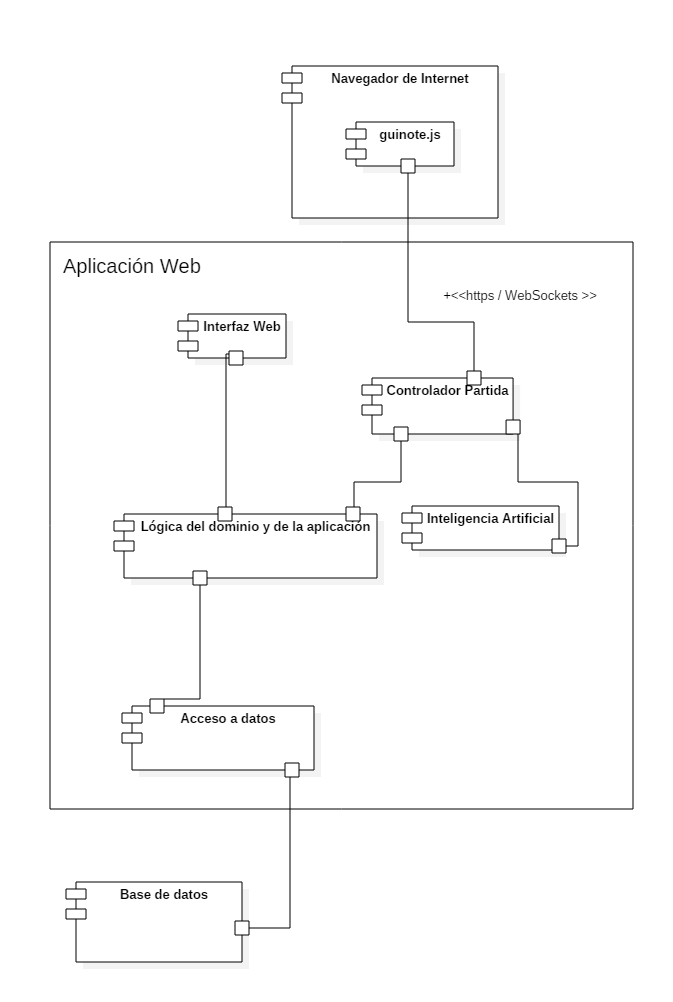
\includegraphics[scale = 0.5]{figuras/diagramaComponentes.png}
\caption{Diagrama de componentes donde se refleja la distribución del sistema}
\label{fig:diagramaComponentes}
\end{figure}

\subsubsection{Base de Datos}

Para la comunicación del sistema con la base de datos se ha utilizado el patrón DAO (Objeto de Acceso a Datos). Para ello se han implementado una serie de objetos VO que representan la información guardada de forma persistente y unos objetos DAO que abstraen las operaciones con el JDBC mediante métodos de Java. Para mayor seguridad de los datos, todos los posibles usos de la base se realizan a través de una interfaz que proporciona los métodos necesarios además de ofrecer un \textit{pool} de conexiones para aumentar la velocidad de la interacción cuando haya múltiples usuarios.\\

Dado el gran número de clases empleado en la implementación del modelo, su representación se ha realizado mediante diferentes diagramas de clases enfocados en las diferentes funcionalidades de la base .
\begin{figure}[H]
\centering
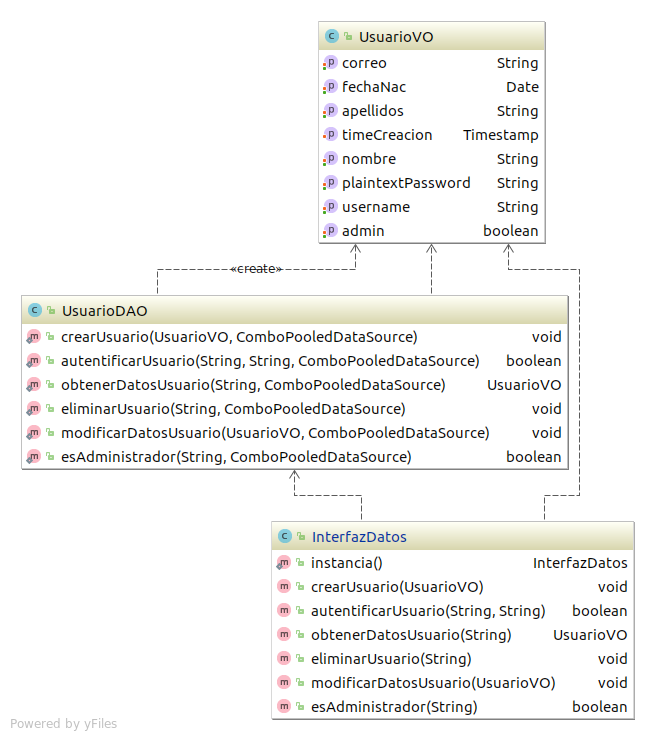
\includegraphics[scale = 0.5]{figuras/base_datos/clasesUsuario.png}
\caption{Diagrama de clases para la funcionalidad de usuario}
\label{fig:diagramaClasesUsuario}
\end{figure}
\begin{figure}[H]
\centering
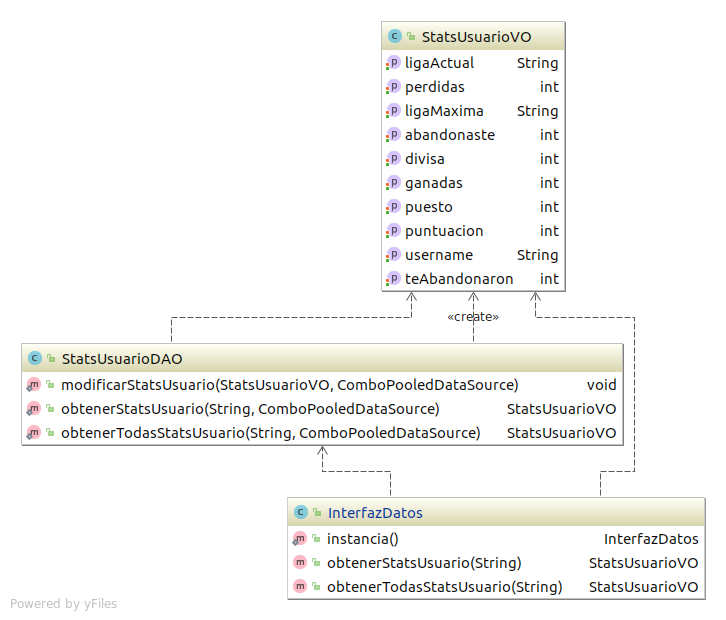
\includegraphics[scale = 0.5]{figuras/base_datos/clasesStats.png}
\caption{Diagrama de clases para la funcionalidad de las estadísticas del usuario}
\label{fig:diagramaClasesStats}
\end{figure}
\begin{figure}[H]
\centering
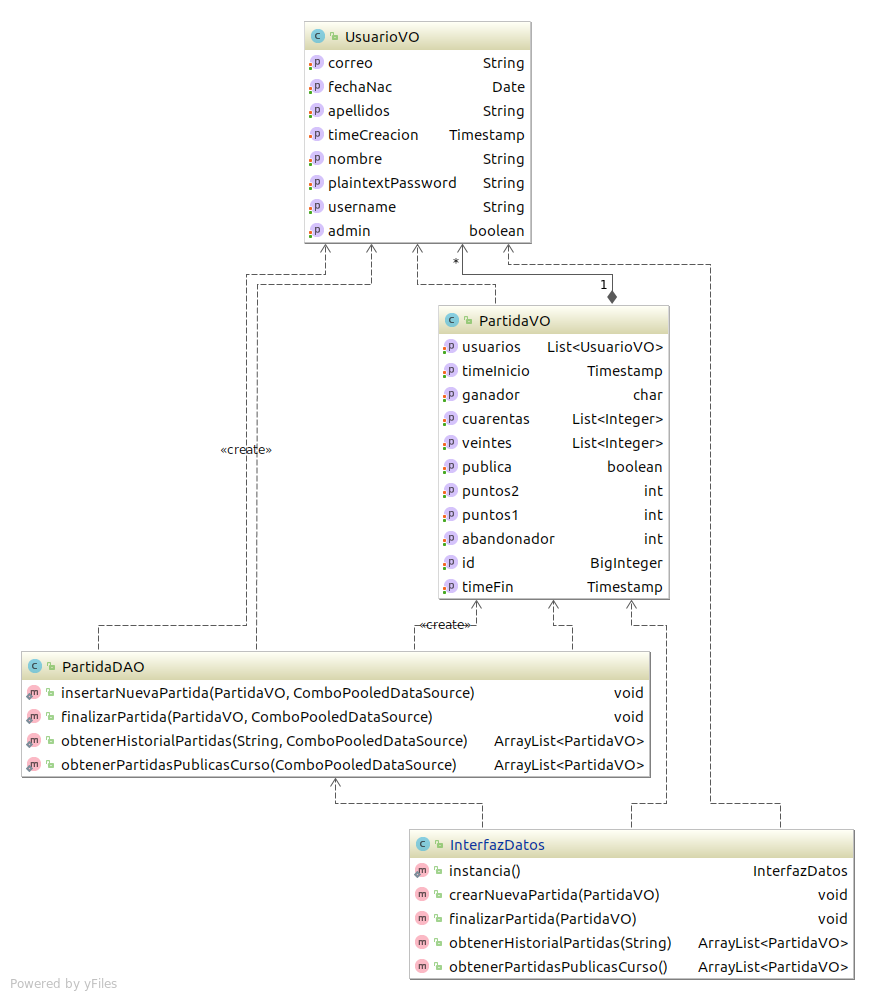
\includegraphics[scale = 0.5]{figuras/base_datos/clasesPartida.png}
\caption{Diagrama de clases para la funcionalidad de partida}
\label{fig:diagramaClasesPartida}
\end{figure}
\begin{figure}[H]
\centering
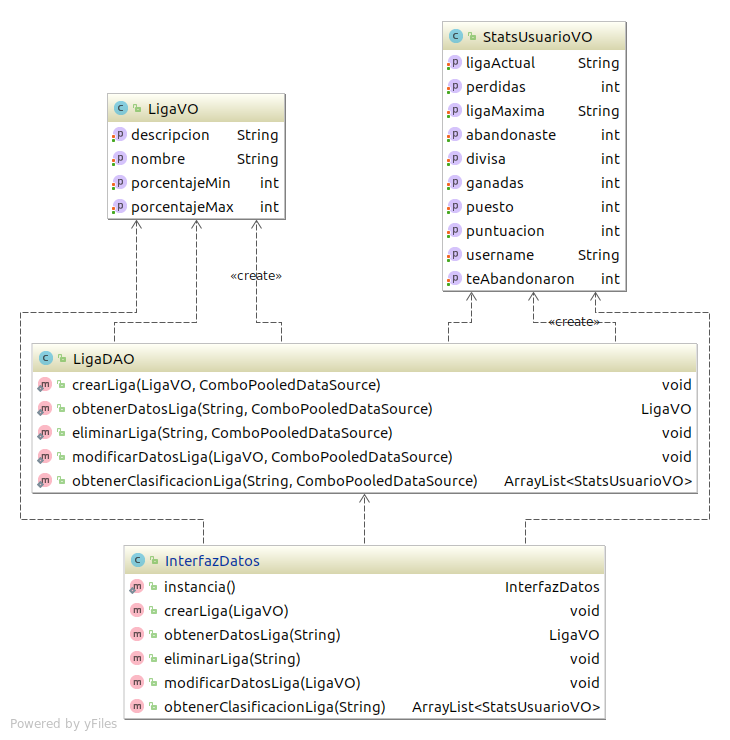
\includegraphics[scale = 0.5]{figuras/base_datos/clasesLiga.png}
\caption{Diagrama de clases para la funcionalidad de liga}
\label{fig:diagramaClasesLiga}
\end{figure}
\begin{figure}[H]
\centering
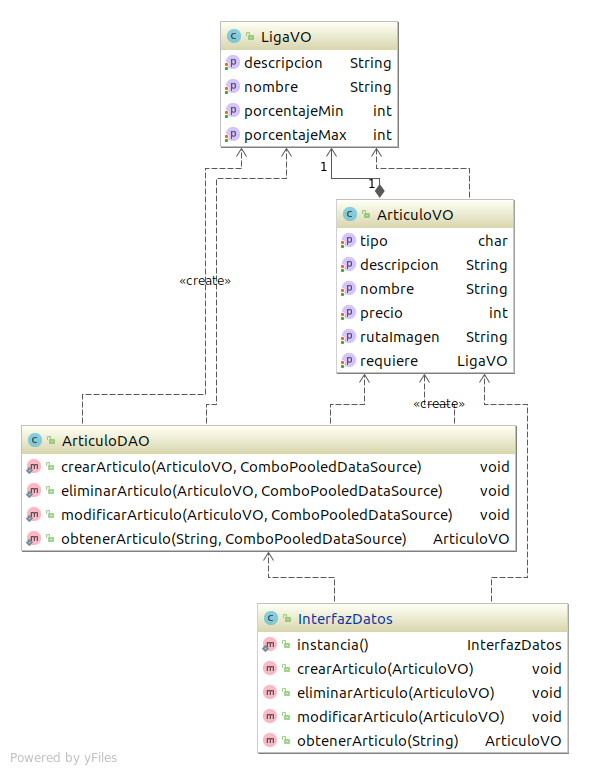
\includegraphics[scale = 0.5]{figuras/base_datos/clasesArticulo.png}
\caption{Diagrama de clases para la funcionalidad de artículo}
\label{fig:diagramaClasesArticulo}
\end{figure}
\begin{figure}[H]
\centering
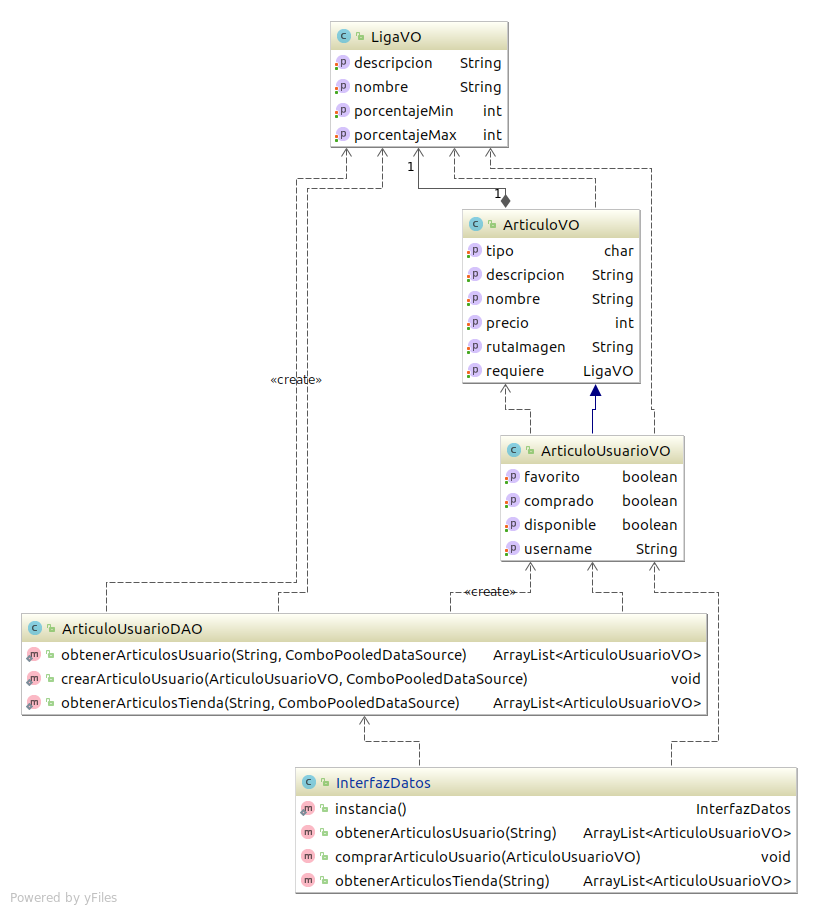
\includegraphics[scale = 0.5]{figuras/base_datos/clasesArticuloUsuario.png}
\caption{Diagrama de clases para la funcionalidad de los artículos de usuario}
\label{fig:diagramaClasesArticuloUsuario}
\end{figure}
\subsection{Tecnologías elegidas}
\begin{itemize}
\item \textbf{Interfaz de la partida en el navegador web}. La interfaz del juego consiste en una única pantalla donde los jugadores que participan en la partida en curso se comunican. Se implementa utilizando JavaScript y Phaser. Phaser es un framework para desarrollo de juegos en HTML5 basado en la tecnología JavaScript.  \\ Se ha decidido utilizar JavaScript por la sencillez a la hora de ser visualizado en un navegador y se incorpora a la perfección con HTML5. Se ha barajado la posibilidad de utilizar Flash pero se descarta por estar obsoleta y porque algunos navegadores ya no lo soportan. También se podría haber utilizado Unity pero no se ha llevado a cabo por tener una curva de aprendizaje muy complicada.
\item \textbf{Capa de comunicación de la partida}. Es el servicio que está por debajo de la partida encargado de notificar las acciones de los jugadores al resto. Además comprueba que el transcurso de la partida es correcto, como si de un coordinador se tratara. Se utiliza lenguaje Java, ya que es un servicio Web e irá desplegado a través de un archivo .war. Además, facilita la comunicación con la tecnología WebSockets, que es la que se ha escogido para comunicar en tiempo real el navegador con el controlador. Se ha decidido WebSockets por tener una curva de aprendizaje sencilla ya que se utilizará para enviar mensajes desde el navegador al controlador. Se integra perfectamente con Java. \\
Se ha descartado utilizar Sockets.io ya que va ligado a Node.js, que es una tecnología más novedosa pero que el equipo desconoce por completo, aprenderla supone un número de horas extras y se desconoce si es una tecnologia viable para la aplicación a desarrollar.
\item \textbf{Interfaz Web}. Se implementa en HTML 5 y se utiliza  JSP y Servlets para la generación de contenido dinámico y procesamiento de formularios, respectivamente. Se trata de una tecnología poco actual pero de la cuál el equipo de desarrollo tiene cierta experiencia, por lo que se asegura la calidad del servicio.
\item \textbf{Lógica y dominio de la aplicación}. Implementado en Java para favorecer la interoperabilidad con la interfaz web.
\item \textbf{Acceso a los datos}. Se utilizan objetos de tipo implementados en Java. De esta manera se cumple el patrón "Modelo - Vista - Controlador".
\item \textbf{Base de datos}. Se utiliza un Sistema Gestor de Bases de Datos relacional, ya que la principales consultas que se hacen son de tipo JOIN. Se ha decidido utilizar MySQL ya que es un sistema que el equipo domina. La desventaja es que es poco eficiente en comparación con otros como Oracle, pero para el número de usuarios que tendrá la aplicación es suficiente con dicho gestor.
\end{itemize}

\subsubsection{BackEnd}

Para la implementación de la lógica del juego se ha análizado el dominio del problema y se ha realizado un primer diseño de clases de análisis. Posteriormente se ha implementado objeto a objeto el diseño inicial y al mismo tiempo actualizando el diagrama de clases.

\begin{figure}[H]
\centering
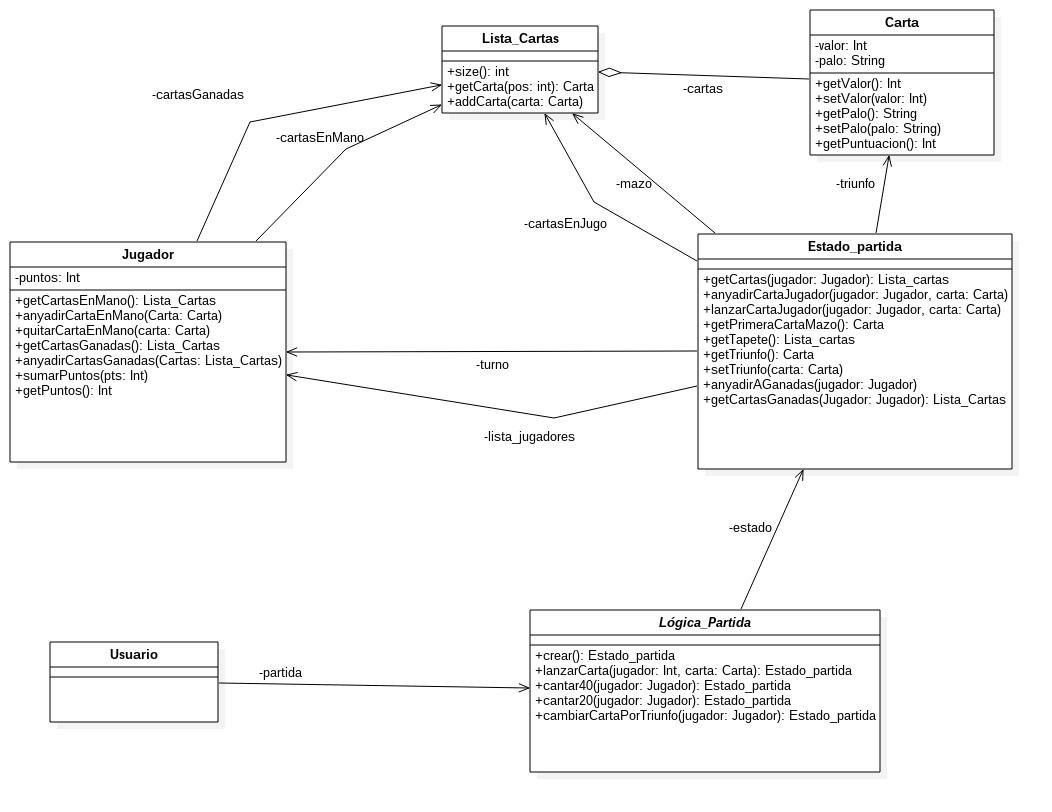
\includegraphics[scale = 0.5]{figuras/logica_juego/diagramaClasesDisenyo.png}
\caption{Diagrama de clases en la fase de análisis del problema}
\label{fig:diagramaClasesLogicaJuegoInicial}
\end{figure}

\begin{figure}[H]
\centering
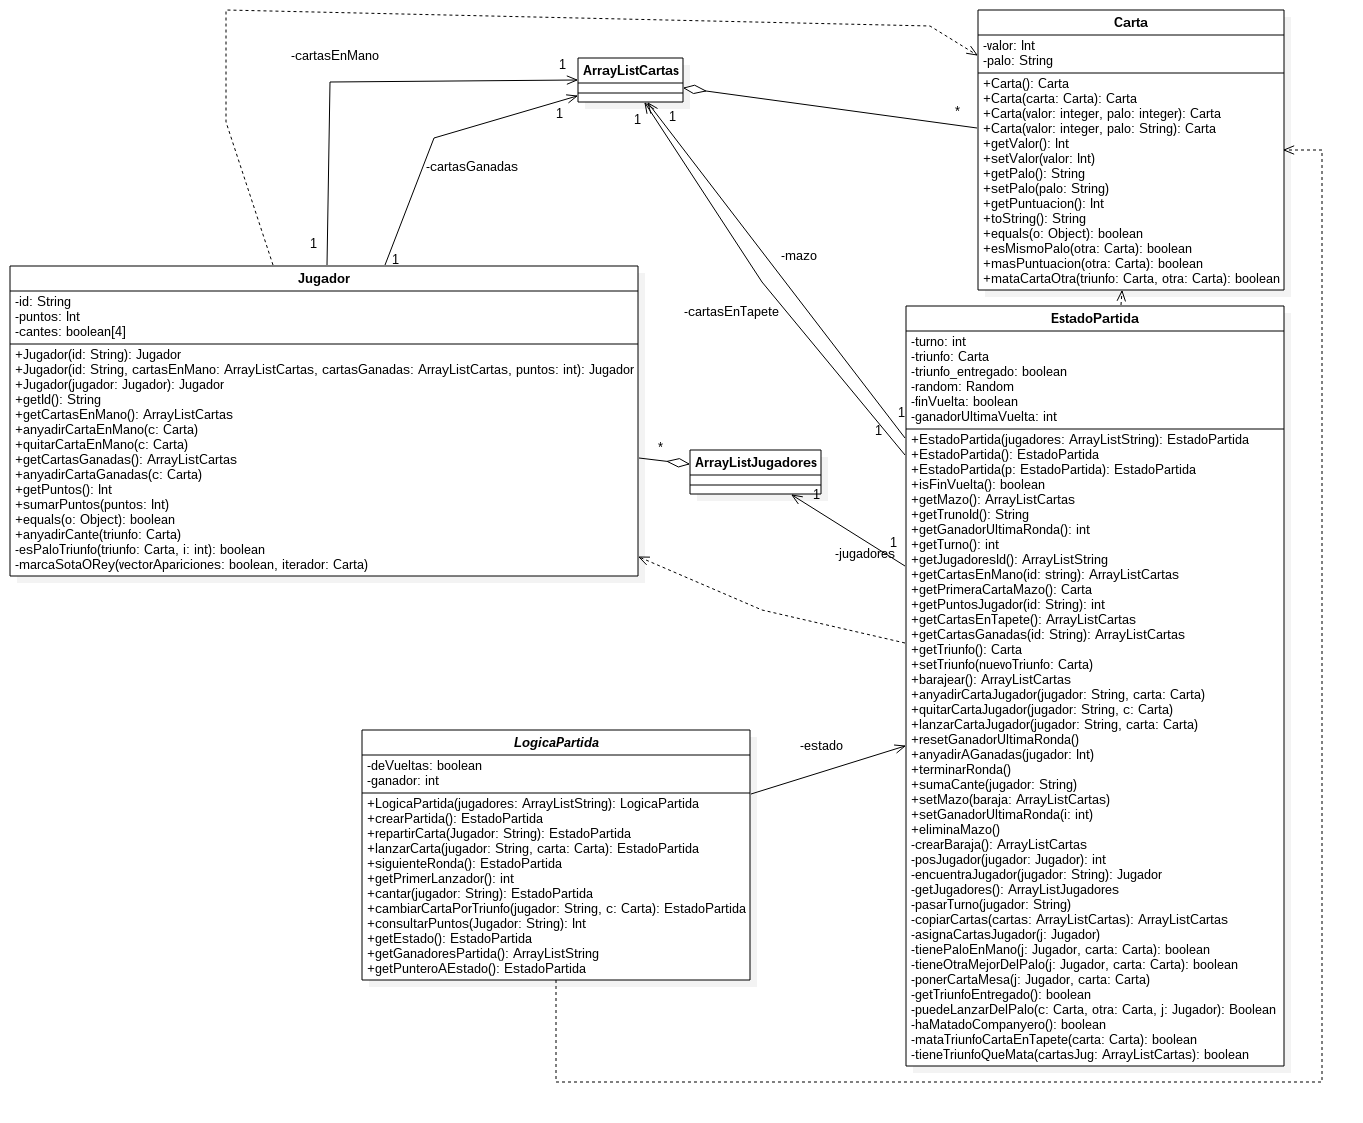
\includegraphics[scale = 0.5]{figuras/logica_juego/diagramaClasesImplementacion.png}
\caption{Diagrama de clases final}
\label{fig:diagramaClasesLogicaJuegoFinal}
\end{figure}

\subsection{Despliegue}
La aplicación se pone en marcha en un servidor Tomcat, ya que permite la instalación de aplicaciones web en formato .war. Se distinguen dos aplicaciones diferentes: la que da soporte a la lógica de la aplicación y la encargada de coordinar una partida en curso. Ambas se comunican indirectamente a través de la base de datos y están coordinadas. \\
La base de datos es relacional ya que se necesitan muchas consultas de los datos almacenados y para cada partida hay varias inserciones o actualización de los datos almacenados. El sistema gestor de la base de datos va a ser MySQL porque se ahorran costes al ser un SGBD de código abierto y no tener que adquirir una licencia de pago. Además, el equipo cuentan con experiencia en el diseño e implementación de bases de datos utilizando MySQL. \\
La razón por la que no se ha elegido otro SGBD de código abierto son los problemas que presenta RDS Aurora. Otros SGBD como PostgreSQL son más exigentes en recursos y, por lo tanto, el coste es mayor sin repercutir un beneficio real sobre la aplicación ya que se considera que MySQL es más que suficiente para una aplicación de estas características.
Otra alternativa era Oracle pero debido al alto coste de la licencia no se ha escogido. \\
El patrón de diseño utilizado para la comunicación del sistema con la base de datos es \textit{façade} ya que permite dividir el sistema completo en dos o más subsistemas consiguiendo un alto desacoplamiento de la base de datos y el juego. De esta forma, se puede dividir mejor el trabajo de forma independiente entre los equipos para poder llevar a cabo un diseño e implementación top-down.

\subsection{Interfaz}
La interfaz, como se ha dicho previamente, se ha desarrollado utilizando la herramienta Phaser, basada en JavaScript. Se ha implementado de manera que sea fácilmente modificable ya que a lo largo de la producción del software se han de introducir cambios, por lo que se han parametrizado la mayoría de las funciones en medida de lo posible.

Una de las principales decisiones de diseño que se han tenido que llevar a cabo es como representar a cada jugador. Se ha hecho de manera que cada jugador tiene su posición como referencia y la interfaz es capaz de representar al resto en función de éste. Como hay un máximo de 4 jugadores, la interfaz toma cada posición como un rol,  teniendo todos los roles los mismos parámetros simulando un patrón de diseño Strategy, para facilitar la integración. El diagrama de clases de la figura \ref{fig:clasesInterfazJuego} muestra la implementación de la interfaz. Aunque en JavaScript no haya clases como tal, se ha aprovechado la sintaxis UML para visualizar las diferentes partes.

\begin{figure}
  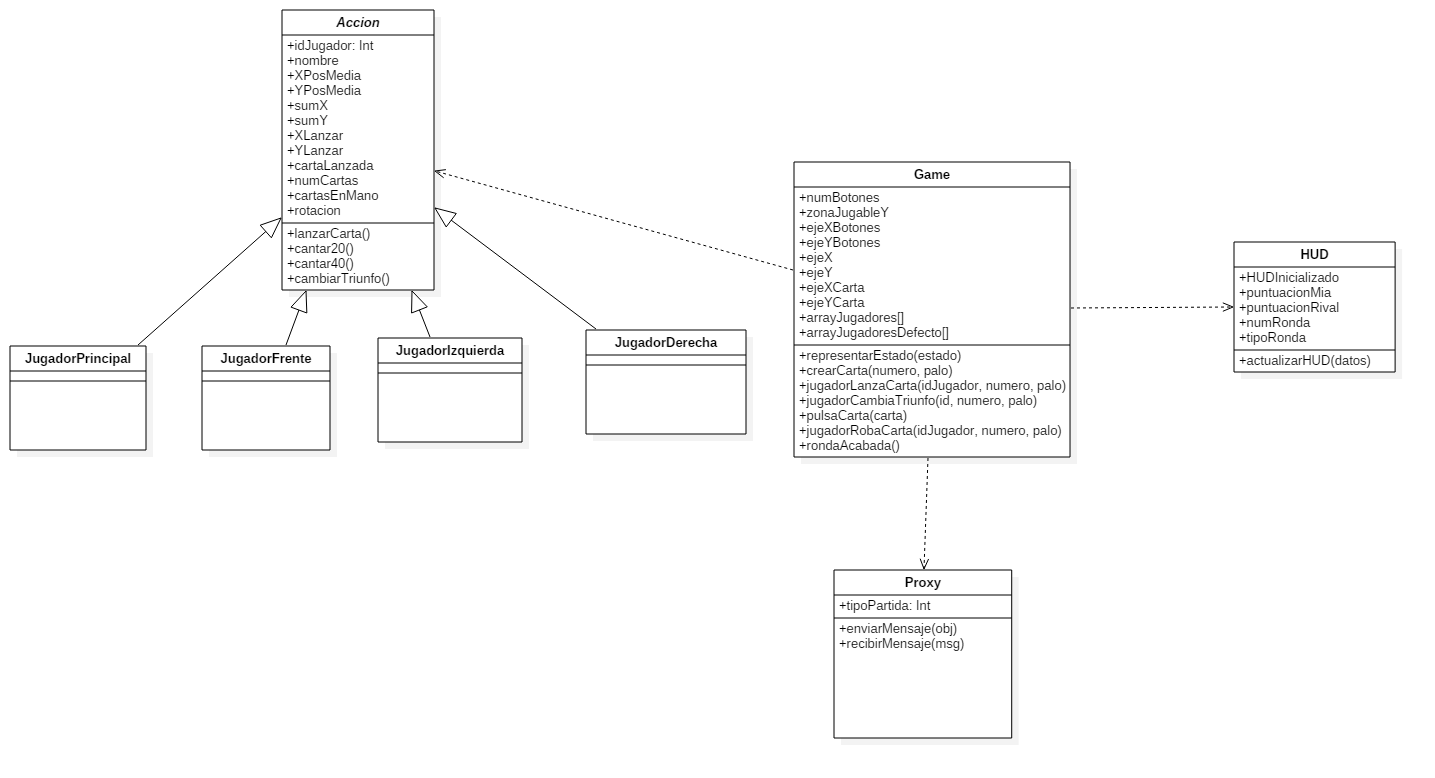
\includegraphics[width=\linewidth]{figuras/clasesInterfazJuego.png}
  \caption{Diagrama de clases de la interfaz de juego}
  \label{fig:clasesInterfazJuego}
\end{figure}

Otra decisión de diseño que sobre la que se ha reflexionado ha sido acerca de la comunicación entre la interfaz y el controlador de la partida. La tecnología que se ha escogido han sido WebSockets como se ha dicho previamente. Dicha tecnología permite únicamente comunicarse a través del paso de mensajes, por lo que se ha decidido que los mensajes sean en formato JSON para que sean fácilmente legibles para ambos extremos de la comunicación.

La aplicación web que no se corresponda con la parte jugable, es decir, el perfil del usuario, la vista del historial de partidas, ligas, torneos, etc. se implementa con JSP y servlets. Se puede observar el mapa de navegación de la aplicación en la figura \ref{fig:mapaDeNavegacion}.

\begin{figure}
  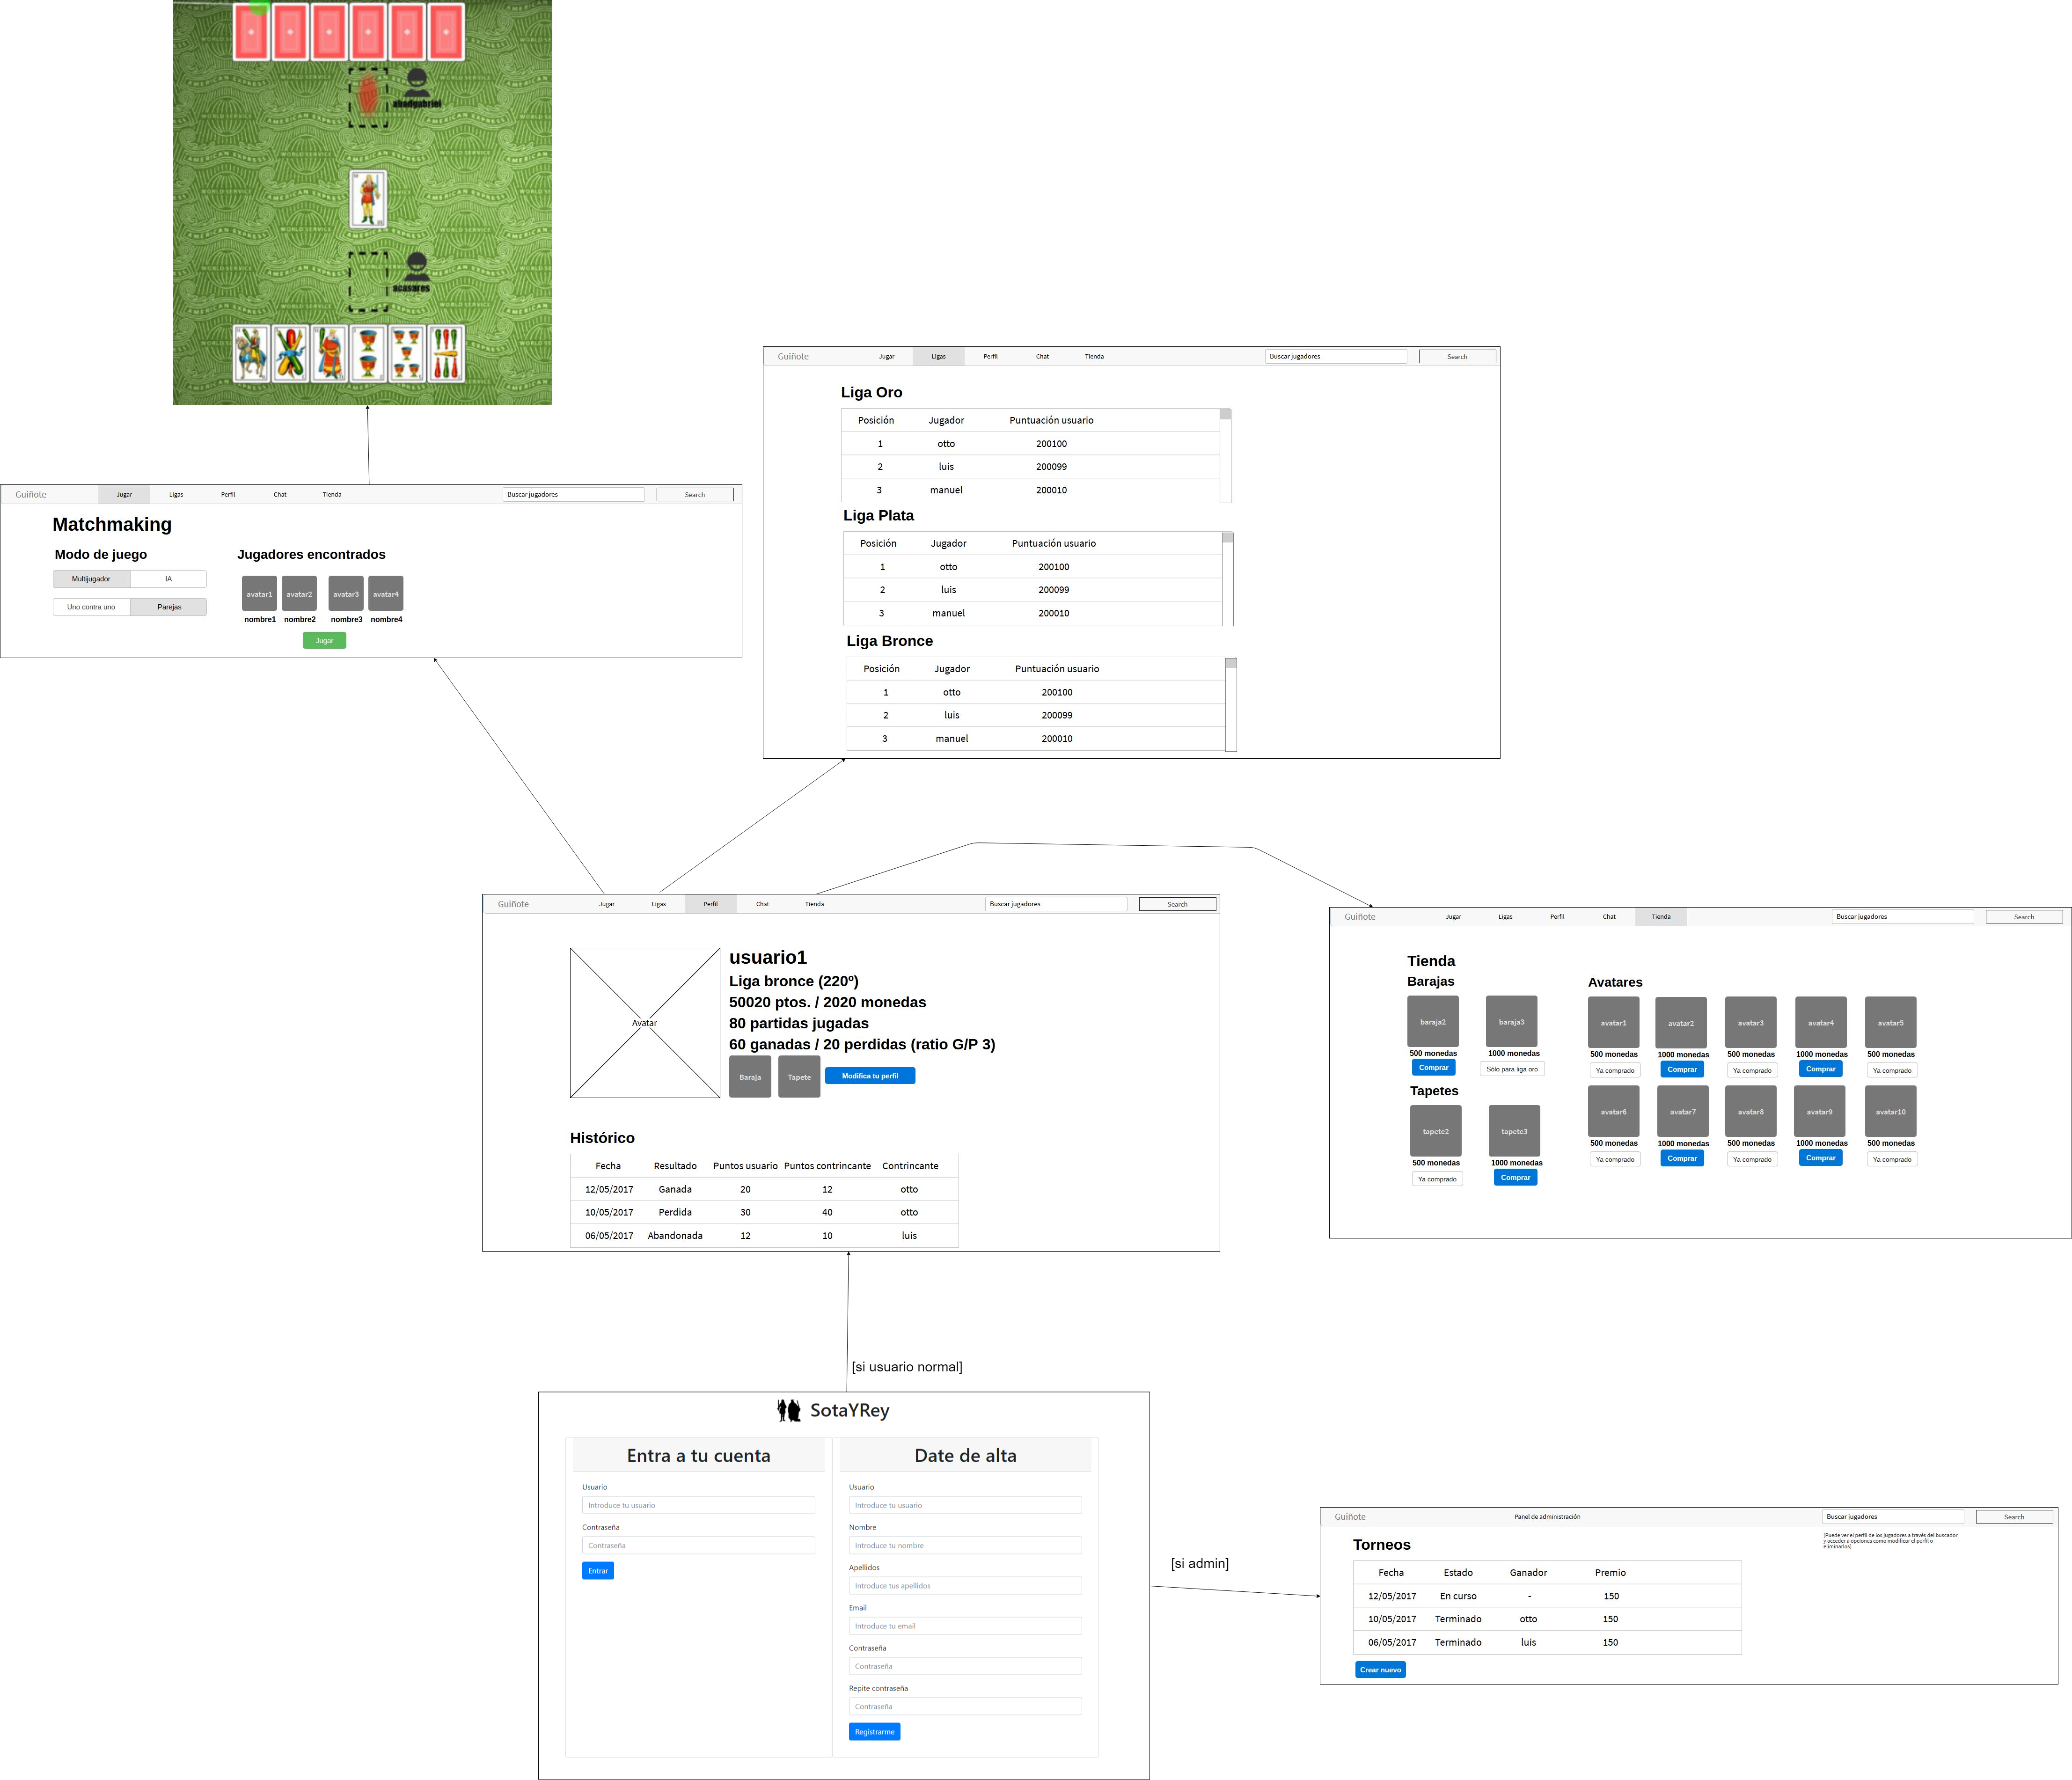
\includegraphics[width=\linewidth]{figuras/mapaNavegacion.png}
  \caption{Mapa de navegación}
  \label{fig:mapaDeNavegacion}
\end{figure}

%\begin{itemize}
%\item  DIAGRAMA DE DESPLIEGUE DE LA APPLICACIÓN WEB EN 3 CAPAS
%\item \textbf{Diagramas arquitecturales (de módulos, de componentes y conectores, de distribución), patrones de diseño y estilos arquitecturales que se aplicarán. Las interfaces (de módulos y de componentes) son especialmente importantes. También lo son los protocolos de comunicación entre componentes.}
%\item \textbf{Tecnologías elegidas (lenguajes de programación, componentes que se integrarán, API web externas con las que se conectará etc.)--ya está--.}

%\item \textbf{Otros aspectos técnicos de interés (p.ej. si hay base de datos si va a ser SQL,  si algunas de las operaciones van a ser asíncronas o no, si se van a usar tecnologías web, cómo se van a considerar los requisitos de seguridad o de prestaciones, cómo y dónde se harán las instalaciones y despliegues etc.)}
%\end{itemize}
%\textbf{Hay que justificar todas las decisiones de diseño. Esto exige contestar a dos preguntas sobre cada decisión: ¿qué alternativas se barajaron? y ¿por qué se eligió una y no las otras?}
